%--------------------------------------------------------------------------
%	PACKAGES AND OTHER DOCUMENT CONFIGURATIONS
%--------------------------------------------------------------------------
\documentclass[11pt,a4paper]{article}
\usepackage[utf8]{inputenc}
\usepackage[english]{babel}
\usepackage[T1]{fontenc}
\usepackage{amsmath}
\usepackage{amsfonts}
\usepackage{amssymb}
\usepackage{graphicx}
\usepackage{lmodern}
\usepackage[left=2cm,right=2cm,top=2.2cm,bottom=2.2cm]{geometry}

\usepackage{fancyhdr} % Required for custom headers
\usepackage{lastpage} % Required to determine the last page for the footer
\usepackage{extramarks} % Required for headers and footers
\usepackage[usenames,dvipsnames]{color} % Required for custom colors
\usepackage{graphicx} % Required to insert images
\usepackage{caption}
\usepackage{subcaption}
\usepackage{listings} % Required for insertion of code
\usepackage{courier} % Required for the courier font
\usepackage{verbatim}
\usepackage{multirow}
\usepackage{eurosym}
\usepackage[squaren,Gray]{SIunits}
\usepackage{url}
\usepackage{hyperref}
\usepackage{multicol}
\usepackage{listings}

% Margins
%\topmargin=-0.45in
%\textwidth=6.5in
%\textheight=9.8in
\headsep=0.25in

% Set up the header and footer
%\pagestyle{fancy}
%\rhead{\firstxmark} % Top right header
%\lfoot{\lastxmark} % Bottom left footer
%\cfoot{} % Bottom center footer
%\rfoot{Page\ \thepage\ /\ \protect\pageref{LastPage}} % Bottom right footer
%\renewcommand\headrulewidth{0.3pt} % Size of the header rule
%\renewcommand\footrulewidth{0.3pt} % Size of the footer rule

\setlength\parindent{0pt} % Removes all indentation from paragraphs

%--------------------------------------------------------------------------
%	CODE INCLUSION CONFIGURATION
%--------------------------------------------------------------------------

\definecolor{MyDarkGreen}{rgb}{0.0,0.4,0.0} % This is the color used for comments
\lstloadlanguages{C} % Load C syntax for listings, for a list of other languages supported see: ftp://ftp.tex.ac.uk/tex-archive/macros/latex/contrib/listings/listings.pdf

\begin{document}
	
%--------------------------------------------------------------------------
%	TITLE PAGE
%--------------------------------------------------------------------------
\begin{titlepage}
\newcommand{\HRule}{\rule{\linewidth}{0.5mm}} % Defines a new command for the horizontal lines, change thickness here
\centering % Center everything on the page
 
%	HEADING SECTIONS
\null
%\vspace{1cm}
\textsc{\Large Université Catholique de Louvain}\\  [0.3cm] % Name of your university/college
\textsc{\large INGI1131 - Computer Language Concepts}\\ [0.7 cm]% Major heading such as course name [0.3cm] [0.5cm]
%\textsc{\large Minor Heading}\\[0.5cm] % Minor heading such as course title


%	TITLE SECTION
\HRule \\[0.2cm]
{ \LARGE \bfseries Zombieland\\%[0.4cm] % Title of your document
\large \bfseries Course Project} \\[0.2cm]
\HRule \\[0.2cm]

% PHOTO
 
\begin{figure}[!h]
	\begin{center}
	%2048 × 1364
		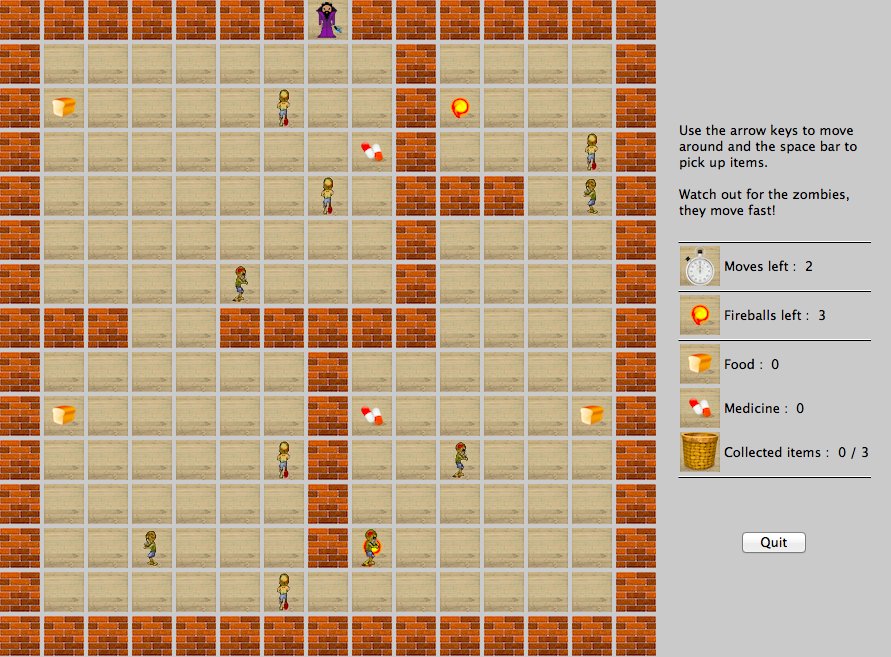
\includegraphics[width=\textwidth]{screenshot.PNG}
	\end{center}
\end{figure}


\emph{\textbf{Abstract} Following an explosion of secret U.S. government laboratories, fast and fearless living beings with a thirst for human blood have invaded the planet. Few survivors have been hiding in a secret place, but they are starting to run out of victuals. A ``brave'' has been designated to collect some. To assist him in this task, we have implemented a simulator that will help him to take all the possible unexpected events into account. Zombies have indeed been studied for a while, so that we are now able to precisely tell you how they move and behave...}\\[0.9cm]


%	AUTHOR SECTION
\begin{multicols}{2}
\large
\begin{centering}
\end{centering}
{\begin{tabular}{lll}
\textit{Group 43}  : & Lena Peschke & 58261100\\
        		     & Mélanie Sedda & 22461100 \\
\end{tabular}}

\normalsize
{\begin{tabular}{ll}
\textit{Professor}  : & Peter Van Roy \\
\textit{TAs} 		: & Zhongmiao Li \\
					  & Manuel Bravo \\
\end{tabular}}
\\[1cm]
\end{multicols}

%	DATE SECTION
{\normalsize \today}\\[0.6cm] % Date, change the \today to a set date if you want to be precise





\newpage

\end{titlepage}

%--------------------------------------------------------------------------
%	TABLE OF CONTENTS
%--------------------------------------------------------------------------

%\pagenumbering{gobble}
%\clearpage
%\thispagestyle{empty}
%\tableofcontents
%\clearpage
%\pagenumbering{arabic}

%--------------------------------------------------------------------------
%	CONTENT
%--------------------------------------------------------------------------

\section*{The game}

The room the brave has to enter contains food, medicine and packs of three bullets. He can kill a zombie with one bullet and can only leave the room if he has collected a certain number of objects (i.e. food + medicine). Our simulator takes four arguments : the map of the room, the number of bullets the brave initially has with him, the percentage of the objects in the room he has the collect and the number of zombies present (default values are used if the user does give any input).

\paragraph{Percentage of objects} If the percentage is $< 0$ (resp. $ > 100$), we transform it into $0$ (resp. $100$).

\paragraph{Number of zombies} We have decided to limit the number of zombies to the number of empty cells on the map, because it would be suicidal to enter a room with more zombies. The zombies can nonetheless still stand on a cell containing an item. 

\paragraph{Moves} The brave and the zombies are moving one after another. When the brave has made $2$ moves, all of the zombies can make $3$ moves at the same time and, when they are done, the brave can move again. Displacements and pickups are considered as moves while killing is not. We decided that the zombies destroy an item $20\%$ of the time when they can. 

\paragraph{Pickups} If the the number of objects needed to leave the room is out of reach for the brave (because the zombies have destroyed some), the brave automatically loses. 

\paragraph{Kills} A brave automatically kills a zombie if he has at least one bullet and if the zombie his in the cell in front of him. However, if he is running out of bullets and if the zombie is facing him, the zombie will automatically kill him. Furthermore, the zombie automatically kills the brave if the brave is in the cell in front of him and isn't facing him.

\section{Architecture and design}

We have identified some port objects that we would need. The main ones are the brave and the zombies, with one port object per zombie. To interact with the map, we also decided to create one port object per cell because it was a quite effective approach. To manage and synchronize the turns of the brave and the zombies, we also created a controller. The functions relative the each entities are located in separated files. Furthermore, we have a file for the GUI and a file for the launch of the game. To implement the interactions between all these entities, we made a component and several state diagrams. Since the codes of the port objects are quite self speaking and always following the same pattern  we will only briefly describe what each port object does (NB : we also sometimes used unbound variables to enforce atomicity in the interaction).

Here is the pattern :
\begin{lstlisting}[basicstyle=\ttfamily\footnotesize]
case Mode
of Mode_1 then ...
	case Msg
	of Msg_1 then ....
	...
	[] Msg_n then ...
	else we ignore the message, but it never happens
	end
...	
[] Mode_m then ...
else we ignore the message, but it never happens
end
\end{lstlisting}
 
	
We have decided to make the ports of the controller, the cells and the brave known by everybody. All of the zombie's ports are known by the controller, and a cell knows the port of a zombie that is one it.

\paragraph{Controller}
The controller has to tell the brave and to the zombies when it is their turn. It knows when a zombie is dead, so it doesn't warn him in this case.  It also has to decide when the brave couldn't win anymore because there are to few objects left in the room. 

\paragraph{Cell}
The room is a grid of cells. Each cell knows which item and person is on it. If it is the brave, it knows his facing direction and the number of bullets he has (this is important for the management of the kills). If it hosts a zombie, it knows his facing direction and his port (also important for the kills).

\paragraph{Brave}
depends on the player

no shooting

bullets no items, because of combats

no mandatory taking

door enabled if count equal or superior to goal

3 times : scout + enter + quit

\paragraph{Zombies}
AI : try moving 3 turns in the same direction, destroy objects 20 \% of the time, change direction randomly if obstacle. If brave, attempt to kill her.

2 times : enter + quit, to avoid overlap between zombies playing in the same turn


\section{Concurrency issues}
synchronization of the turns between the brave and the zombies

synchronization between the zombies : not on the same cell


\section{Miscellaneous}
QTk?

    
\section*{Conclusion}
We think that your game should fulfill the requirements and hope that it will provide you some help to survive.
    
\end{document}